When thinking about finite tree automata, it is often desirable to have a
few simple examples in mind to compare classes.  We have collected a few
such examples here.

\subsection{Equalities Vs. Recursion}

\subsubsection{All-equal lists}

Not all classes of automata permit free interaction of recursion and
equality constraints; as such, these classes may not be able to describe the
language of all-equal lists: $\set{ [], [A], [A,A], [A,A,A], \ldots }$ for
any $A$.  Note, however, that for a fixed, regular tree $A$, the set of
all-equal lists of $A$ is a regular tree language.  The difficulty emerges
when we wish to describe all-equal lists over an unbounded number of
possible elements.

\subsubsection{Markovian-equal lists}

A generalization of the above, consider the language of lists composed of
regions of size at least two whose elements are equal, for example:
$[A,A,B,B,B]$ or $[A,A,A,B,B,C,C,D,D,D,D]$.  Rigid tree automata will not be
able to describe such a class due to the need for unboundedly many
equivalence classes.

\subsection{Opacity}

Consider the sets of trees described by
%
\begin{center}\begin{tabular}{cc}
    $\set{ f(g(X,Y),g(Z,X)) \middle\vert X,Y,Z \in \mathcal{T}(\Sigma)}$
  & $\set{ f(W,g(A,B)) \middle\vert A,B,W \in \mathcal{T}(\Sigma) \wedge A\vert_1 = B\vert_2 }$
  \\
    \begin{tikzpicture}
      \Tree [.f [.g X Y ] [.g Z X ] ]
    \end{tikzpicture}
  & \begin{tikzpicture}
      \Tree [.f W [.g$_{11=21}$ A B ] ]
    \end{tikzpicture}
\end{tabular}\end{center}
%
These descriptions are clearly (given their comprehension form) amenable to
classification by Opaque constraints.  Their intersection is $\set{
f(g(A,B),g(C,A)) \middle\vert A,B,C \in \mathcal{T}(\Sigma) \wedge C\vert_1
= A\vert_2 }$, which can be made amenable to Opaque classification only if
we are able to unfold $\mathcal{T}(\Sigma)$ for $A$ and $C$.  While we can
do this for regular trees over finite $\Sigma$, in general what we are
calling here $A$ will actually be trees accepted by a particular state, so
we can only describe this intersection with Opaque constraints if we are
able to unfold the description of that state.  In general, that unfolding
process might not terminate.
%
\Note{I would feel a lot better if somebody checked this.}

\subsection{Necessarily Overlapping}
\label{sec:tree-sepex:necessaryoverlap}

\begin{wrapfigure}{r}{1in}\centering\begin{tikzpicture}
  \Tree [.f$_{1=22}$ X [.g$_{1=2}$ X X ] ]
\end{tikzpicture}\end{wrapfigure}
The tree in the figure to the right is a small example of a structure which
necessarily involves overlapping constraints, assuming that the nodes
$X$ are drawn from an infinite set of trees; if there are merely finitely
many possibilities, then the constraints may be pushed into the state
label.  Specifically, because we must constrain positions $1$, $21$ and $22$
to be equal, we are obligated to have at least one of $21$ and $22$ as
constraint paths in the automata, and then either the other, which overlaps,
or the constraint $1=2$ at position $2$, which again overlaps.  However,
this structure is amenable to Opaque description, as shown.
